\documentclass[11pt,a4paper]{scrartcl}
\usepackage[utf8]{inputenc}
\usepackage[utf8]{inputenc}
\usepackage[ngerman]{babel}
\usepackage[T1]{fontenc}
\usepackage{amsmath}
\usepackage{amsfonts}
\usepackage{amssymb}
\usepackage{mathtools}
\usepackage{graphicx}
\usepackage{multirow}
\usepackage{fancyhdr}
\usepackage{float}
\pagestyle{fancy}
\usepackage[a4paper,
			bottom=1.7in,
			left=1.2in,
			right=1.2in,
			top=1.2in,
			headsep = 35pt]
	{geometry}
\usepackage{tikz}% for drawing automata etc
\usetikzlibrary{automata,arrows,chains,shapes.misc,scopes,petri,matrix,patterns}
%\usepackage[x11names]{xcolor}
%\usepackage[parfill]{parskip}
\usepackage{array}
%\usepackage{gslist}
%\usepackage{subfigure}
\usepackage{subcaption}
\usepackage{enumitem}
\usepackage{algpseudocode} %for pseudocode
\usepackage[siunitx,european,straightlabels,straightvoltages]{circuitikz} %draw Electrical Circuits

\ctikzset{bipoles/text rotate/.initial=0,% <=new key
rotation/.style={\circuitikzbasekey/bipoles/text rotate=#1},% style for ease introduction in code
}

% code from pgfcircbipoles.sty
\makeatletter
\pgfcircdeclarebipole{}{\ctikzvalof{bipoles/ammeter/height}}{ammeter}{\ctikzvalof{bipoles/ammeter/height}}{\ctikzvalof{bipoles/ammeter/width}}{
    \def\pgf@circ@temp{right}
    \ifx\tikz@res@label@pos\pgf@circ@temp
        \pgf@circ@res@step=-1.2\pgf@circ@res@up
    \else
        \def\pgf@circ@temp{below}
        \ifx\tikz@res@label@pos\pgf@circ@temp
            \pgf@circ@res@step=-1.2\pgf@circ@res@up
        \else
            \pgf@circ@res@step=1.2\pgf@circ@res@up
        \fi
    \fi

    \pgfpathmoveto{\pgfpoint{\pgf@circ@res@left}{\pgf@circ@res@zero}}       
    \pgfpointorigin \pgf@circ@res@other =  \pgf@x  \advance \pgf@circ@res@other by -\pgf@circ@res@up
    \pgfpathlineto{\pgfpoint{\pgf@circ@res@other}{\pgf@circ@res@zero}}
    \pgfusepath{draw}

    \pgfsetlinewidth{\pgfkeysvalueof{/tikz/circuitikz/bipoles/thickness}\pgfstartlinewidth}

        \pgfscope
            \pgfpathcircle{\pgfpointorigin}{\pgf@circ@res@up} % change this if you want to touch the wires
            \pgfusepath{draw}       
        \endpgfscope    

    \pgftransformrotate{\ctikzvalof{bipoles/text rotate}}% <= magic line
    \pgfsetlinewidth{\pgfstartlinewidth}

    \pgfsetarrowsend{latex}
    \pgfpathmoveto{\pgfpoint{\pgf@circ@res@other}{\pgf@circ@res@down}}
    \pgfpathlineto{\pgfpoint{-1.06\pgf@circ@res@other}{1.06\pgf@circ@res@up}} % change this if you want to touch the wires
    %\pgfusepath{draw} % comment this if you don't need the diagonal arrow
    \pgfsetarrowsend{}


    \pgfpathmoveto{\pgfpoint{-\pgf@circ@res@other}{\pgf@circ@res@zero}}
    \pgfpathlineto{\pgfpoint{\pgf@circ@res@right}{\pgf@circ@res@zero}}
    %\pgfusepath{draw} % comment this if you don't need the diagonal arrow


    \pgfnode{circle}{center}{\textbf{A}}{}{}
}

% code from pgfcircbipoles.sty
\pgfcircdeclarebipole{}{\ctikzvalof{bipoles/voltmeter/height}}{voltmeter}{\ctikzvalof{bipoles/voltmeter/height}}{\ctikzvalof{bipoles/voltmeter/width}}{
    \def\pgf@circ@temp{right}
    \ifx\tikz@res@label@pos\pgf@circ@temp
        \pgf@circ@res@step=-1.2\pgf@circ@res@up
    \else
        \def\pgf@circ@temp{below}
        \ifx\tikz@res@label@pos\pgf@circ@temp
            \pgf@circ@res@step=-1.2\pgf@circ@res@up
        \else
            \pgf@circ@res@step=1.2\pgf@circ@res@up
        \fi
    \fi

    \pgfpathmoveto{\pgfpoint{\pgf@circ@res@left}{\pgf@circ@res@zero}}       
    \pgfpointorigin \pgf@circ@res@other =  \pgf@x  \advance \pgf@circ@res@other by -\pgf@circ@res@up
    \pgfpathlineto{\pgfpoint{\pgf@circ@res@other}{\pgf@circ@res@zero}}
    \pgfusepath{draw}

    \pgfsetlinewidth{\pgfkeysvalueof{/tikz/circuitikz/bipoles/thickness}\pgfstartlinewidth}

        \pgfscope
            \pgfpathcircle{\pgfpointorigin}{\pgf@circ@res@up} % change this if you want to touch the wires
            \pgfusepath{draw}       
        \endpgfscope    

    \pgftransformrotate{\ctikzvalof{bipoles/text rotate}}% <= magic line
    \pgfsetlinewidth{\pgfstartlinewidth}

    \pgfsetarrowsend{latex}
    \pgfpathmoveto{\pgfpoint{\pgf@circ@res@other}{\pgf@circ@res@down}}
    \pgfpathlineto{\pgfpoint{-1.06\pgf@circ@res@other}{1.06\pgf@circ@res@up}} % change this if you want to touch the wires
    %\pgfusepath{draw} % comment this if you don't need the diagonal arrow
    \pgfsetarrowsend{}


    \pgfpathmoveto{\pgfpoint{-\pgf@circ@res@other}{\pgf@circ@res@zero}}
    \pgfpathlineto{\pgfpoint{\pgf@circ@res@right}{\pgf@circ@res@zero}}
    %\pgfusepath{draw} % comment this if you don't need the diagonal arrow


    \pgfnode{circle}{center}{\textbf{V}}{}{}
}
\makeatother


\author{Alexander Halbarth}

\setlist[enumerate]{label=\alph*)}
%\setlist[itemize]{label=$\rightarrow$}


 \tikzset{
endbox/.style={pattern=crosshatch,minimum height=.8cm}}

%\partfont{\centering}
\newcommand\tab[1][1cm]{\hspace*{#1}}
\usepackage{framed, color}


\newcommand{\UE}{Übung 2}
\newcommand{\name}{Fragenkatalog zum Überprüfungsgespräch Elektrotechnische Grundlagen}
\title{\textbf{Fragenkatalog zum Überprüfungsgespräch Elektrotechnische Grundlagen Übungen für TI 2017 - \UE}}


\newcommand{\ul}[1]{\underline{#1}} % für unterstreichen von einzelnen Symbolen einfach \ul x - wenn man ein Wort unterstrichen will \ul{wort}
%\newcommand\sy[1]{{\underline{\ifmmode\mathtt{#1}\else\texttt{#1}\fi}}} % ähnlich wie \ul - verwendet aber andere Schriftart
%\newlistt\sys\sy{\hspace{1pt}}{}{}{^} % identisch zu \sy, \sys{wort} unterstreicht aber jeden Buchstaben einzeln und \sy{wort} unterstreicht das ganze Wort
% (sofern das Alphabet nur aus einzelnen Zeichen besteht ist \sys{wort} einfacher


%no line indent
\setlength\parindent{0pt}

\fancyhead[R]{\UE}
\fancyhead[L]{\name}
\fancyfoot[C]{\thepage}

\renewcommand{\footrulewidth}{0pt}
\renewcommand{\headrulewidth}{0.5pt}


\begin{document}
\maketitle
\textbf{Frage 1: Was machst Du gerade im Labor und welchen Sinn hat das?}\\
\textbf{Frage 2: Nenne die Grundgrößen der Elektrotechnik, deren Formelzeichen und Einheit.}\\
Spannung $U[$Volt $V]$, Strom $I[$Ampere $A]$, Widerstand $R[$Ohm $\Omega]$,Leistung $P[$Watt $W]$\\
\textbf{Frage 2: Elektrische Spannung: Nenne Definition (nicht über das Ohmsche Gesetz!), Formelzeichen und Einheit}\\
Die potentielle Energie(=Arbeit) die durch eine Ladungstrennung gespeichert wurde.\\
\textbf{Frage 2: Elektrischer Strom: Nenne Definition (nicht über das Ohmsche Gesetz!), Formelzeichen und Einheit}\\
Ladung eines Elektrons $Q_e=1,6 \cdot 10^{-19}C=1,6 \cdot 10^{-19}A\cdot s$\\
$\frac{6*10^{18}e^-}{1s}=\frac{As}{1s} \rightarrow 6*10^{18}$ Elektronen fließen durch einen Leiter pro Sekunde bei $1A$\\
\textbf{Frage 2: Elektrischer Widerstand: Nenne Definition (nicht über das Ohmsche Gesetz!), Formelzeichen und Einheit}\\
Ist eine Materialeigenschaft\\
Beispiel Kupfer $17m\Omega \cdot mm^2/m$\\
\textbf{Frage 2: Elektrische Leistung: Nenne Definition, Formelzeichen und Einheit}\\
Die in einer Zeitspannung umgesetzte elektrische Energie bezogen auf die Zeitspanne.\\
\textbf{Frage 2: Wie berechnet man die elektrische Leistung in einem Gleichstromkreis?}\\
$U=R \cdot I \rightarrow P=U \cdot I$\\
\textbf{Berechne die an einem Widerstand entstehende Leistung, wenn durch ihn bei einer Spannung von $2V$ ein Strom von $3A$ fließt.}\\
$6W$\\
\textbf{Frage 2: Welcher Phasenwinkel besteht zwischen Wechselspannung und Wechselstrom an einem idealen Kondensator?}\\
Die Spannung folgt dem Strom um $90^\circ=\pi/2$ nach. (eigentlich $-90^\circ$)\\
\textbf{Welcher Phasenwinkel besteht zwischen Wechselspannung und Wechselstrom an einer idealen Induktivität?\\
(Die Vorzeichen brauchen nicht explizit angegeben zu werden, müssen aber verglichen werden).}\\
Der Strom folgt der Spannung nach um $90^\circ=\pi/2$ nach. (eigentlich $+90^\circ$)\\
\textit{Gehen in entgegengesetzte Richtungen!}\\
\textbf{Frage 2: Formuliere das ohmsche Gesetz.}\\
$U=R*I$\\
\textbf{Berechne den Widerstand, wenn bei einem Strom von $3A$ eine Spannung von $3V$ abfällt.}\\
\textbf{Frage 2: Berechne den Strom, wenn an einem Widerstand von $5\Omega$ eine Spannung von $10V$ abfällt.}\\
\textbf{Frage 2: Berechne die Spannung, wenn durch einen Widerstand von $10\Omega$ ein Strom von $5A$ fließt. }\\
\textbf{Frage 2: Formuliere die Kirchhoffschen Regeln.}\\
\textbf{Auf welchem physikalischen Grundprinzip beruhen diese?}\\
\textit{Energieerhaltung}\\
Maschenregel: Summe aller Spannungen muss 0 ergeben.\\
Knotenregel: Summe aller Ströme muss 0 ergeben.\\
\textbf{An einem Spannungsteiler liegen $9V$. Am oberen Widerstand liegen $6V$ an.}\\
\textbf{Berechne die Spannung am unteren Widerstand.}\\
\textbf{Frage 2: In einen Stromknoten mit drei Leitungen fließen aus einer Leitung $2A$ hinein und aus einer anderen Leitung $3A$ hinein. Was geschieht in der dritten Leitung?}\\
\textbf{Frage 2: Nenne die Zehnerpotenzen zu den SI - Präfixen Nano, Milli und Mikro. Nenne die SI - Präfixe zu: $10^3, 10^6, 10^9$}\\
\begin{tabular}{|l|l|l|}
\hline
\textbf{Präfix} & \textbf{Zeichen} & \textbf{Faktor}\\
\hline\hline
Piko   & p  & $10^{-12}$\\
\hline
Nano   & n  & $10^{-9}$\\
\hline
Mikro  & $\mu$ & $10^{-6}$\\
\hline
Milli  & m  & $10^{-3}$\\
\hline
Zenti  & c  & $10^{-2}$\\
\hline
Dezi   & d  & $10^{-1}$\\
\hline\hline
Deka   & da & $10^{1}$\\
\hline
Hekto  & h  & $10^{2}$\\
\hline
Kilo   & k  & $10^{3}$\\
\hline
Mega   & M  & $10^{6}$\\
\hline
Giga   & G  & $10^{9}$\\
\hline
Tera   & T  & $10^{12}$\\
\hline
\end{tabular}\\
\newpage
\textbf{Frage 3: Skizziere Kurvenform und Spektrum eines Sinus / symmetrischen Rechteck / Impuls - Signals.\\
Hinweis: Du legst fest, was genau Du unter "`Impuls"' verstehst. Das Spektrum muss zur angegebenen Kurvenform passen!}\\
\begin{figure}[H]
\minipage{0.32\textwidth}
  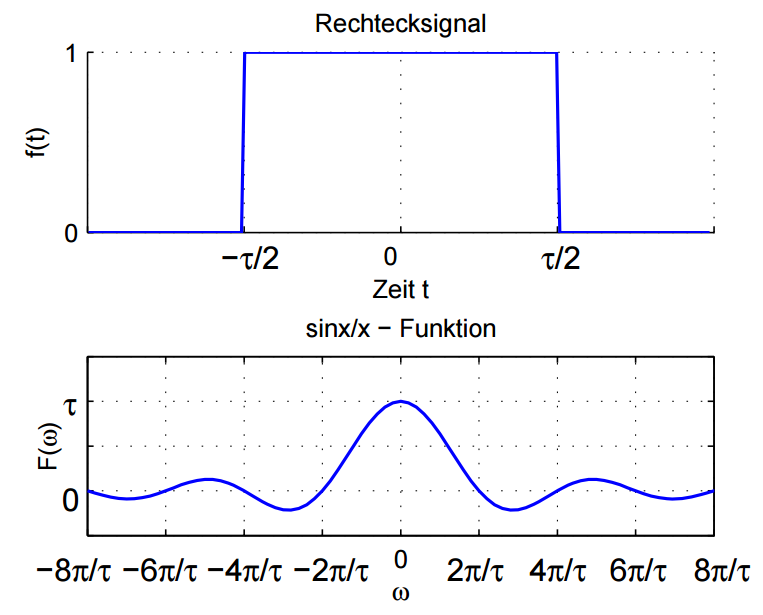
\includegraphics[width=\linewidth]{rechteck.png}
\endminipage\hfill
\minipage{0.32\textwidth}
  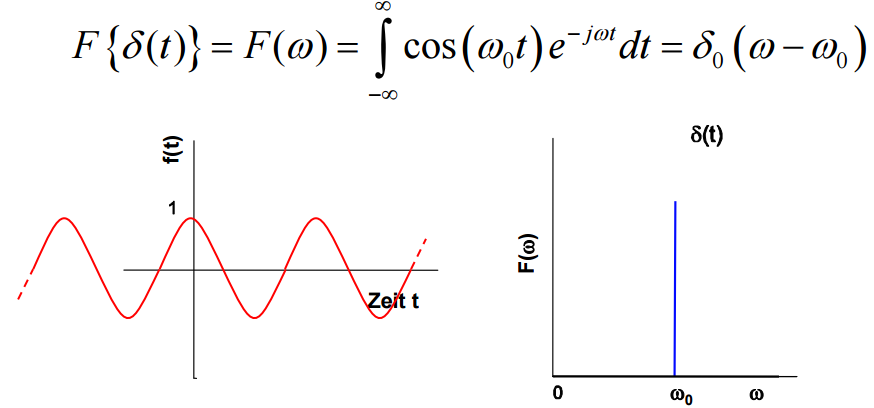
\includegraphics[width=\linewidth]{sinus.png}
\endminipage\hfill
\minipage{0.32\textwidth}
  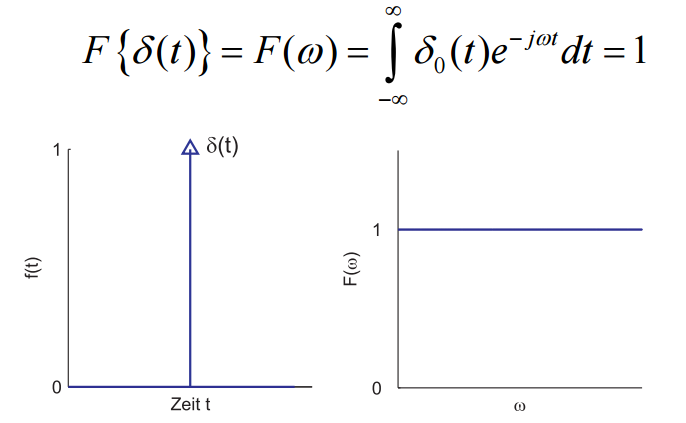
\includegraphics[width=\linewidth]{impuls.png}
\endminipage
\end{figure}
\textbf{Frage 3: Skizziere den Verlauf des Quotienten U / I eines ohmschen Widerstandes}\\
\textbf{Begründe Deine Skizzen durch die Angabe der Berechnungsformeln.}\\
konstant\\
\textbf{Skizziere den Verlauf des Quotienten U / I eines idealen Kondensators} \\
Hyperbel\\
\textbf{Skizziere den Verlauf des Quotienten U / I einer idealen Spule als Funktion der Frequenz.}\\
linear\\
\textbf{Frage 3: Erkläre die Bedeutung von $dB$.}\\
$10\cdot log(\frac{P_1}{P_2})$\\
\textbf{Welches Spannungsverhältnis wird durch $20dB$ ausgedrückt?}\\
$20 \cdot log(\frac{U_1}{U2})=2 \rightarrow U_1=U_2\cdot10^{1}$\\
\textbf{Frage 3: In einen Stromknoten mit drei Leitungen fließen aus einer Leitung $2A$ sinusförmiger $50Hz$ Wechselstrom hinein und aus einer anderen Leitung $3A$ sinusförmiger $50Hz$ Wechselstrom hinein. \\
Kannst Du anhand dieser Angaben berechnen, was in der dritten Leitung geschieht? Begründe Deine Entscheidung!}\\
Nein, da wir die Phasenverschiebungen der einzelnen Leitungen nicht kennen.\\
\textbf{Frage 4: Skizziere die Schaltung eines RC – Hochpassfilters. Gib seine Grenzfrequenz an.}\\
  \begin{circuitikz} \draw
			(0,0) to[V<=$U_{in}$,i^>=$I$] (0,2)
						to[C]    (2,2)
						to[R,v^>=$U_{out}$,*-*] (2,0)
						-- (0,0)
						(2,2)--(2.5,2)
						(2,0)--(2.5,0);
\end{circuitikz}\\
$X_C=R=\dfrac{1}{2\pi \cdot f \cdot C}$\\
$f_G=\dfrac{1}{2\pi \cdot R \cdot C}$\\
\newpage
\textbf{Frage 4: Skizziere die Schaltung eines RC – Tiefpassfilters. Gib seine Grenzfrequenz an.}\\
  \begin{circuitikz} \draw
			(0,0) to[V<=$U_{in}$,i^>=$I$] (0,2)
						to[R]    (2,2)
						to[C,v^>=$U_{out}$,*-*] (2,0)
						-- (0,0)
						(2,2)--(2.5,2)
						(2,0)--(2.5,0);
\end{circuitikz}\\
$X_C=R=\dfrac{1}{2\pi \cdot f \cdot C}$\\
$f_G=\dfrac{1}{2\pi \cdot R \cdot C}$\\
\textbf{Frage 4: Skizziere die Schaltung eines RL – Hochpassfilters. Gib seine Grenzfrequenz an.}\\
  \begin{circuitikz} \draw
			(0,0) to[V<=$U_{in}$,i^>=$I$] (0,2)
						to[R]    (2,2)
						to[L,v^>=$U_{out}$,*-*] (2,0)
						-- (0,0)
						(2,2)--(2.5,2)
						(2,0)--(2.5,0);
\end{circuitikz}\\
$X_L=R=2\pi \cdot f \cdot L$\\
$f_G=\dfrac{R}{2\pi \cdot L}$\\
\textbf{Frage 4: Skizziere die Schaltung eines RL - Tiefpassfilters. Gib seine Grenzfrequenz an.}\\
  \begin{circuitikz} \draw
			(0,0) to[V<=$U_{in}$,i^>=$I$] (0,2)
						to[L]    (2,2)
						to[R,v^>=$U_{out}$,*-*] (2,0)
						-- (0,0)
						(2,2)--(2.5,2)
						(2,0)--(2.5,0);
\end{circuitikz}\\
$X_L=R=2\pi \cdot f \cdot L$\\
$f_G=\dfrac{R}{2\pi \cdot L}$\\
\textbf{Frage 4: Skizziere die Schaltung eines RLC - Bandpassfilters. (2 Antworten zulässig) Gib seine Mittenfrequenz an.}\\
\begin{circuitikz} \draw
			(0,0) to[V<=$U_{in}$,i^>=$I$] (0,2)
						to[L]    (2,2)
						to[C] (4,2)
						to[R,v^>=$U_{out}$,*-*] (4,0)
						-- (0,0)
						(4,2)--(4.5,2)
						(4,0)--(4.5,0);
\end{circuitikz}\\
$f_0=\dfrac{1}{2\pi\sqrt{C\cdot L}}$\\
\newpage
\textbf{Frage 4: Skizziere das Bode-Diagramm eines RC - Hochpassfilters. Achte auf die korrekte Achsenteilung!}\\
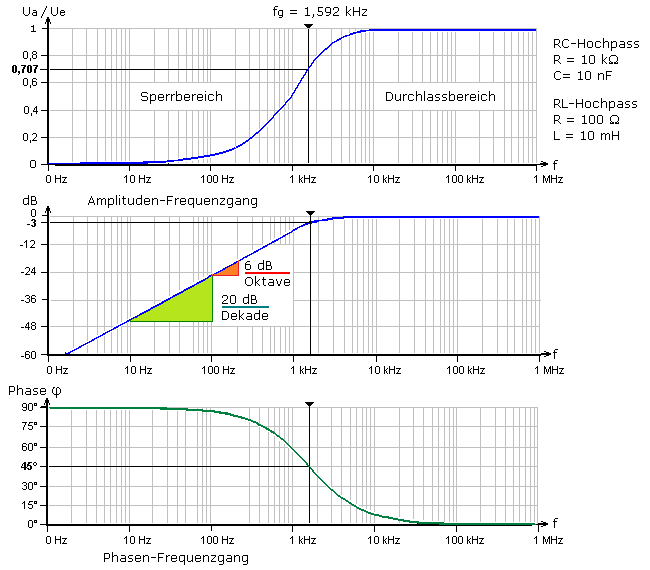
\includegraphics[height=7cm]{hochpass_bode.png}\\
\textbf{Frage 4: Skizziere die Sprungantwort eines Tiefpassfilters 1. Ordnung.}\\
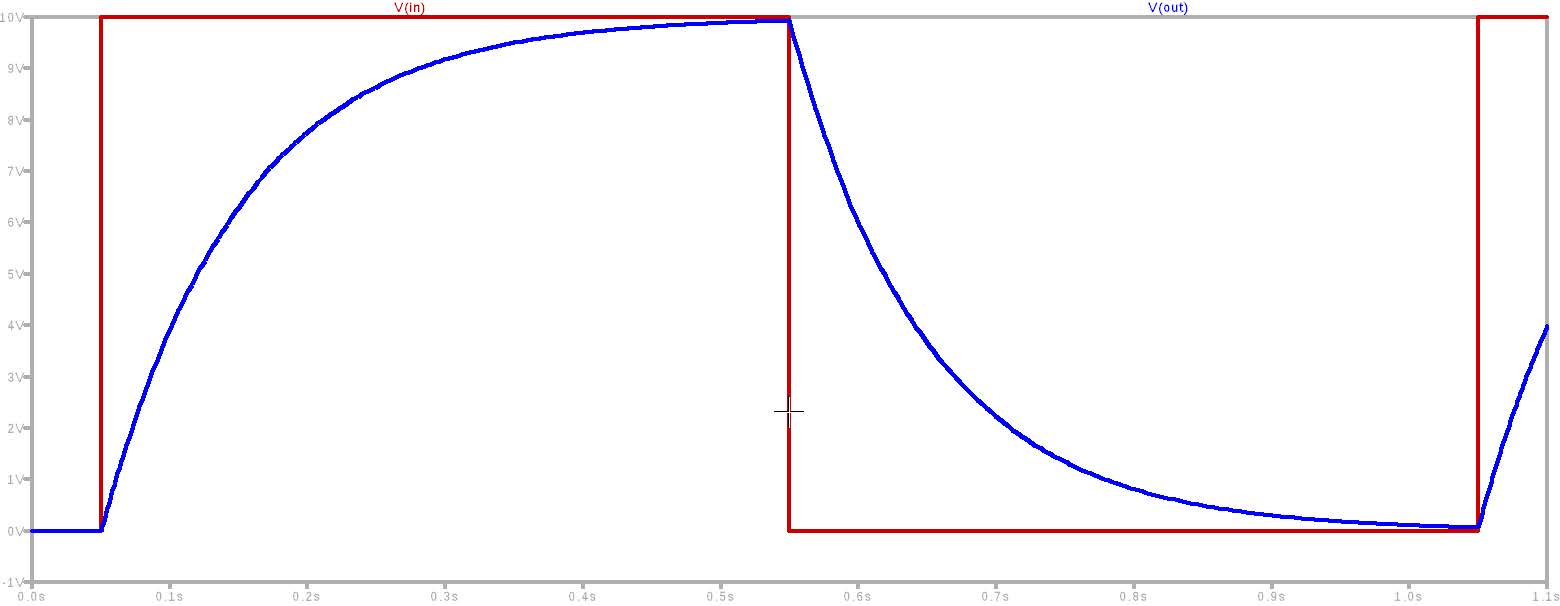
\includegraphics[width=7cm]{sprung_tiefpass.jpg}\\
\textbf{Skizziere die Sprungantwort eines Hochpassfilters 1. Ordnung.}\\
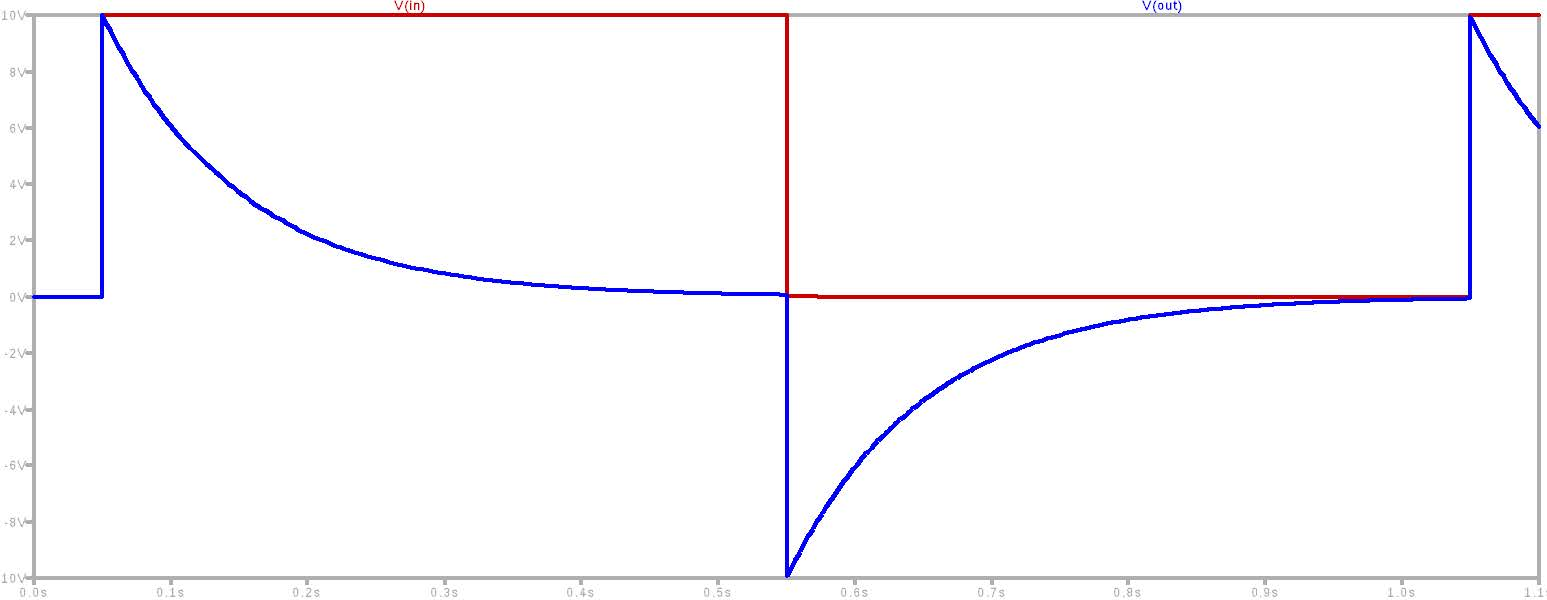
\includegraphics[width=7cm]{sprung_hochpass.jpg}\\
\textbf{Begründe Deine Darstellungen.}\\
\textit{Tiefpass}: Der Kondensator wird geladen bis die Eingangsspannung fast erreicht wird. Ist dieser voll liegt nun die komplette Spannung am Ausgang an.\\
\textit{Hochpass}: Sobald der Kondensator quasi voll geladen auf die Eingangsspannung ist, liegt das selbe Potential am Ausgang an wie auf der Masse.\\
\textbf{Frage 4: Durch welche beiden Messungen lassen sich Filter besonders effektiv charakterisieren?}\\
Sprungantwort und Frequenzverhalten.\\
\textbf{Wie gehst Du dabei praktisch vor?}\\
Rechtecksignal für Sprungantwort.\\
Sinusförmiges Signal für Frequenzverhalten.\\
\textbf{Frage 4: Wie verhält sich die Ausgangsspannung eines Tiefpassfilters bei sinusförmigen Eingangsspannungen mit Frequenzen weit unter der Grenzfrequenz?}\\
Fast genauso wie die Eingangsspannung.\\
\newpage
\textbf{Wie verhält sich die \textcolor[rgb]{0,0,1}{Ausgangsspannung} eines Tiefpassfilters bei \textcolor[rgb]{1,0,0}{rechteckförmigen Eingangsspannungen} mit Periodenzeiten kleiner als die Zeitkonstante?}\\
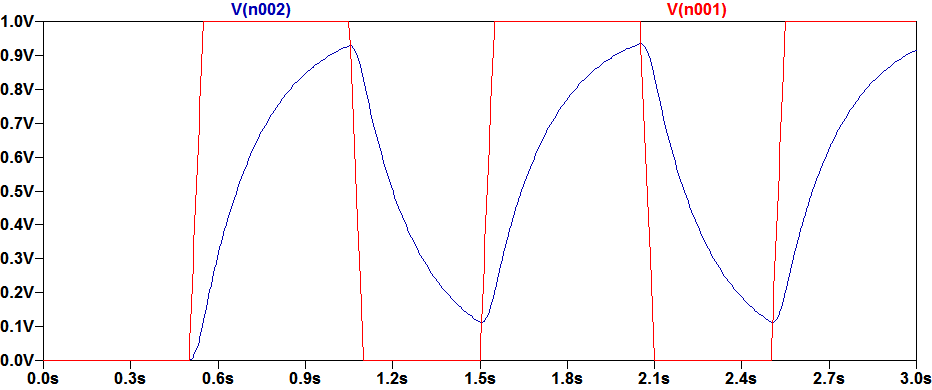
\includegraphics[width=10cm]{TP_Rechteck.png}\\
\textbf{Frage 4: Wie verläuft die Übertragungsfunktion eines Tiefpassfilters bei Frequenzen deutlich höher als die Grenzfrequenz?}\\
Sie werden gedämpft umso weiter von der Grenzfrequenz entfernt.\\
\textbf{Durch welche elektrotechnische Größe wird dieser Verlauf quantifiziert?}\\
Filtersteilheit (Steigung im Bode Diagramm) $\left[\frac{dB}{Dekade}\right]$\\
\textbf{Frage 4: Wie verläuft die Übertragungsfunktion eines Hochpassfilters bei Frequenzen deutlich niedriger als die Grenzfrequenz?}\\
Sie werden gedämpft umso weiter von der Grenzfrequenz entfernt.\\
\textbf{Durch welche elektrotechnische Größe wird dieser Verlauf quantifiziert?}\\
Filtersteilheit (Steigung im Bode Diagramm) $\left[\frac{dB}{Dekade}\right]$\\
\textbf{Frage 5: Welchen Vorteil haben Tiefpassfilter 2. Ordnung gegenüber Tiefpassfiltern 1. Ordnung?}\\
\begin{circuitikz} \draw
			(0,0) to[V<=$U_{in}$,i^>=$I$] (0,2)
						to[L]    (2,2)
						to[C] (4,2)
						to[R,v^>=$U_{out}$,*-*] (4,0)
						-- (0,0)
						(4,2)--(4.5,2)
						(4,0)--(4.5,0);
\end{circuitikz}\\
Abfall der Frequenz um $40dB/Dekade$ statt $20$. Dh. Effektiver\\
Steilere Dämpfung \& höherer Phasengang\\
\textbf{Skizziere die Übertragungsfunktionen im Frequenzbereich.}\\
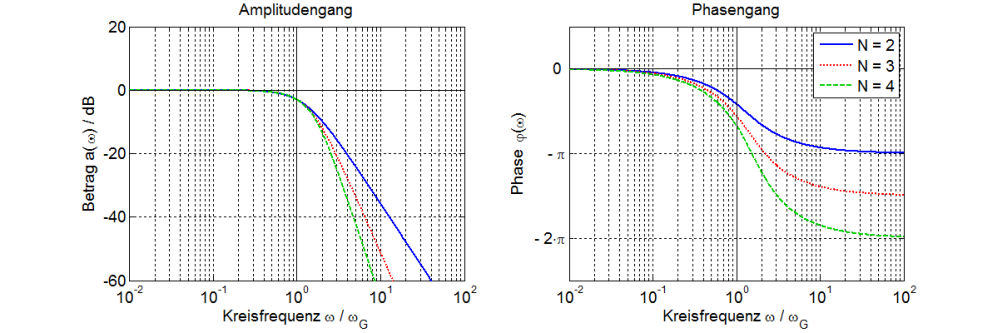
\includegraphics[width=10cm]{tiefpass_2o.png}\\
\newpage
\textbf{Frage 5: Dieses Diagramm zeigt zwei Sprungantworten eines dynamischen Systems 2. Ordnung, beispielsweise eines LCR - Bandpassfilters.\\
Was sagen diese beiden Sprungantworten über die Dämpfung aus?}\\

\begin{figure}[H]
\minipage{0.49\textwidth}
	\begin{center}
	\includegraphics[width=4cm,keepaspectratio]{sprungantwort.jpg}
	\end{center}
\endminipage\hfill
\minipage{0.49\textwidth}
	\begin{center}
	\begin{circuitikz} \draw
				(0,0) to[V<=$U_{in}$,i^>=$I$] (0,2)
						-- (1,2)
						to[R]    (3,2)
			(1,2)	to[C,*-*] (1,0)
						-- (0,0)
						(3,2)--(3.5,2)
						(1,0)--(3.5,0)
			(3,2)	to[L,v^>=$U_{out}$,*-*] (3,0);
	\end{circuitikz}
\end{center}
\endminipage\hfill
\end{figure}

%$\omega = \dfrac{1}{\sqrt{LC}}$

%1. Antwort: $\dfrac{R}{2L}\geq\dfrac{1}{\sqrt{L\cdot C}}$
1. Antwort: Je größer der Widerstand, desto größer die Dämpfung\\
%2. Antwort: $\dfrac{R}{2L} < \dfrac{1}{\sqrt{L\cdot C}}$ 
2. Antwort: Widerstand so klein, dass das System schwingt\\
\textbf{Wie ist das möglich, dass eine negative Spannung auftritt, obwohl nur passive Bauelemente verwendet werden?}\\
Aufgrund des Schwingungsverhaltens zwischen Kondensator und Spule.\\

\end{document}
